\documentclass[aspectratio=169]{beamer}

\usepackage{tikzducks}

\setbeamertemplate{navigation symbols}{}
\setbeamertemplate{background canvas}{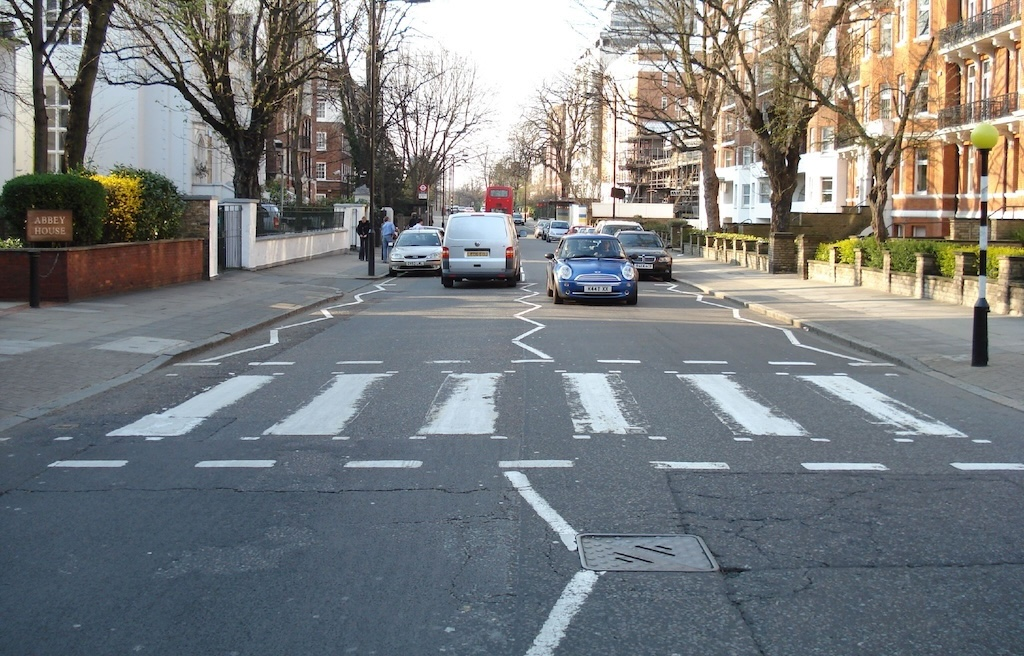
\includegraphics[width=\paperwidth]{Abbey_Road_zebra_crossing,_London_2007-03-31}}
\graphicspath{{include/}}

% trick taken from https://topanswers.xyz/tex?q=1989
\tikzset{
    use page relative coordinates/.style={
        shift={(current page.south west)},
        x={(current page.south east)},
        y={(current page.north west)}
    },
}

\usepackage{xfp}
\ExplSyntaxOn
\let\intmodnn\int_mod:nn
\ExplSyntaxOff

\begin{document}

\begin{frame}<1-300>[label=quack]
  \begin{tikzpicture}[remember picture, overlay,use page relative coordinates]
  
    \ifnum \intmodnn{\thepage}{10} > 5
      \node[anchor=east,xshift=-17cm+\insertoverlaynumber*0.05cm] at (1,0.4) {
\includegraphics[height=3cm,page=1]{walking}};
    \else
      \node[anchor=east,xshift=-17cm+\insertoverlaynumber*0.05cm] at (1,0.4) {
\includegraphics[height=3cm,page=2]{walking}};
    \fi  

    % credit for background image
    \node[white,text width=.8\paperwidth,font=\tiny,align=center] at ([yshift=0.35cm]current page.south) {Image by @m.caimary \href{https://creativecommons.org/licenses/by/2.0/deed.en}{CC BY 2.0} (\url{https://en.wikipedia.org/wiki/File:Abbey_Road_zebra_crossing,_London_2007-03-31.jpg})};

  \end{tikzpicture}
  \pause[600]
\end{frame}

\begin{frame}
  \begin{tikzpicture}[remember picture, overlay,use page relative coordinates]
  
    \node[anchor=east,xshift=-17cm+300*0.05cm] at (1,0.4) {
\includegraphics[height=3cm,page=3]{walking}};

    % credit for background image
    \node[white,text width=.8\paperwidth,font=\tiny,align=center] at ([yshift=0.35cm]current page.south) {Image by @m.caimary \href{https://creativecommons.org/licenses/by/2.0/deed.en}{CC BY 2.0} (\url{https://en.wikipedia.org/wiki/File:Abbey_Road_zebra_crossing,_London_2007-03-31.jpg})};

  \end{tikzpicture}
  \pause[50]
\end{frame}

\begin{frame}
\begin{tikzpicture}
\fill[white] (current page.south west) rectangle (current page.north east);
\end{tikzpicture}
\end{frame}


\againframe<300->{quack}

\end{document}